\documentclass{cumcm}




\begin{document}


\begin{minipage}{0.9\textwidth}
\centering\LARGE\textbf{基于电化学阻抗普法的锂电池SOH预测模型}
\end{minipage}
\begin{abstract}
本题题意在于通过对测试数据充足的锂电池建立SOH模型,找出可测数据与电池SOH之间的关系,并使模型适用于不同的锂电池,进而完成测试数据较少的锂电池SOH预测。本篇论文采用电化学阻抗谱法完成对电池SOH的预测分析。\par
\textbf{电化学阻抗谱法} \quad 研究电池单体的老化规律,从电池寿命的定义、交流阻抗测量条件的制定,到阻抗参数与电池老化规律分析,至最终的SOH算法开发,已有的研究验证了该方法估算电池SOH的可行性。\par
\textbf{针对问题一}\quad 我们首先需要完成对源数据中,电池SOH与循环次数关系曲线、电池内阻与循环次数关系曲线分析,来验证该锂电池满足电化学阻抗谱法的使用条件,然后通过MATLAB拟合出电池内阻与电池SOH的关系曲线,找出电池内阻与电池SOH之间的关系式,从而建立出普适的预测模型,来预测目标数据的电池SOH,并算出预测SOH与真实值的均方根误差,检验模型的准确程度。\par
\textbf{针对问题二} \quad \par
\textbf{关键词} \quad MATLAB \quad 电化学阻抗谱法  \quad 锂电池SOH
\end{abstract}

\newpage
\section{问题重述}
\subsection{问题背景}
电池是一种能量转化与储存的装置,它通过反应可将化学能或物理能转化为电能,从而得到具有稳定电压、长时间稳定供电的电流。作为众多移动终端的动力单元及绿色环保电池的首选,锂离子电池在电池界具有举足轻重的地位,并在各种电子设备中得到了越来越广泛的应用。其在便携式设备、储备电源、卫星、电动汽车等领域,更是具有广阔的前景。
\subsection{问题的提出(题目重述)}
随着使用情况的增多,锂离子电池会逐渐老化,我们通常采用SOH(锂电池放电容量与锂电池额定容量的比值)表示锂离子电池的老化程度。为了保证设备的稳定,预测锂电池的SOH便具有了重要的意义。然而不同类型的锂电池,其测试数据的多少会有不同。要求利用一个测试数据充足的锂电池SOH预测模型,通过数学建模方法转化,完成测试数据较少的锂电池SOH预测。

\begin{itemize}
\item \textbf{任务一} \quad 利用源数据中B0007号锂电池全部循环测试的充放电参数(电压、电流等)建模预测源数据中B0005号锂电池SOH,计算真实SOH值与预测值的均方根误差。
\item \textbf{任务二} \quad 取cell1、cell3、cell7、cell8中前一半数据,结合任务一B0007号锂电池的模型再次建模,对这四种电池中另一半缺失数据的锂电池SOH进行预测,计算真实SOH值与预测值的均方根误差。
\end{itemize}

\section{模型假设}
\begin{enumerate}
\item 在本题所给数据中,环境温度恒为$24^\circ$C,所以外界环境温度对电池SOH的影响不予考虑。
\item 不考虑恒压充电情况。
\item 不考虑充放电电流对电池SOH值影响。
\item 将电池EIS作为电池SOH的两大影响因素。
\end{enumerate}
\section{假设说明}
\begin{enumerate}
\item EIS为电池老化过程中阻抗谱变化。
\item 由参考文献[2]可知,在恒压充电情况下,电池SOH值改变较小,可忽略,仅考虑恒流充电情况。
\item 考虑电池在放电过程中,放电电流、温度等因素较为复杂,而充电过程情况较为稳定,因此选用电池充电电压曲线拟合估算。
\item 由参考文献[2]可知,电池EIS会随着电池老化而发生相应改变,说明EIS变化与电池SOH衰减具有相关性。
\end{enumerate}

\section{方法介绍}
锂离子电池阻抗谱模型基于多孔电极理论和浓溶液理论提出,清华大学$Li zhe$等提出模型从单个粒子、凝聚物、多孔电极三个尺度上逐次建立基于机理的电池阻抗模型,具有较高的精度。首先,在单个粒子的阻抗模型中,通过对频率的小正弦信号的激励下的系统的控制方程的求解来建立阻抗响应,得到的单个粒子阻抗。在凝聚物阻抗和多孔电极阻抗建模中,是通过代表性体积单元来平均微观方程,如用体积平均法平均液相控制方程等,最后得到凝聚物阻抗和多孔电极阻抗,即电化学阻抗谱模型。
\section{问题分析}
对于问题一和问题二,可采用同样的方法进行建模。\par
由题目所给测试数据及所查参考文献,对于锂电池老化机理分析,从锂离子电池众多特性中找到一个或多个可以准确衡量电池性能的参数,显然参数越多越好,越能反映电池内部状态越好。EIS在众多特性参数中脱颖而出,与电池的外特性端电压相比,EIS的各频段对应于相关的电化学反应过程,具有原位、无损反应电池内部电化学反应机理的特点。此外,电池的EIS会随着电池老化而发生相应变化,说明EIS的变化与电池性能退化之间具有相关性,通过电化学阻抗谱模型可以建立电池EIS与电池老化过程中电池内部参数之间的联系,进而了解电池的健康。\cite{1}
\subsection{问题一分析}
本题所给测试数据中,采用循环充放电方式对BOOO7号样本电池老化试验,我们可得出随着循环次数的增加,电池SOH衰减曲线,如图所示:
\begin{figure}[H]
\centering
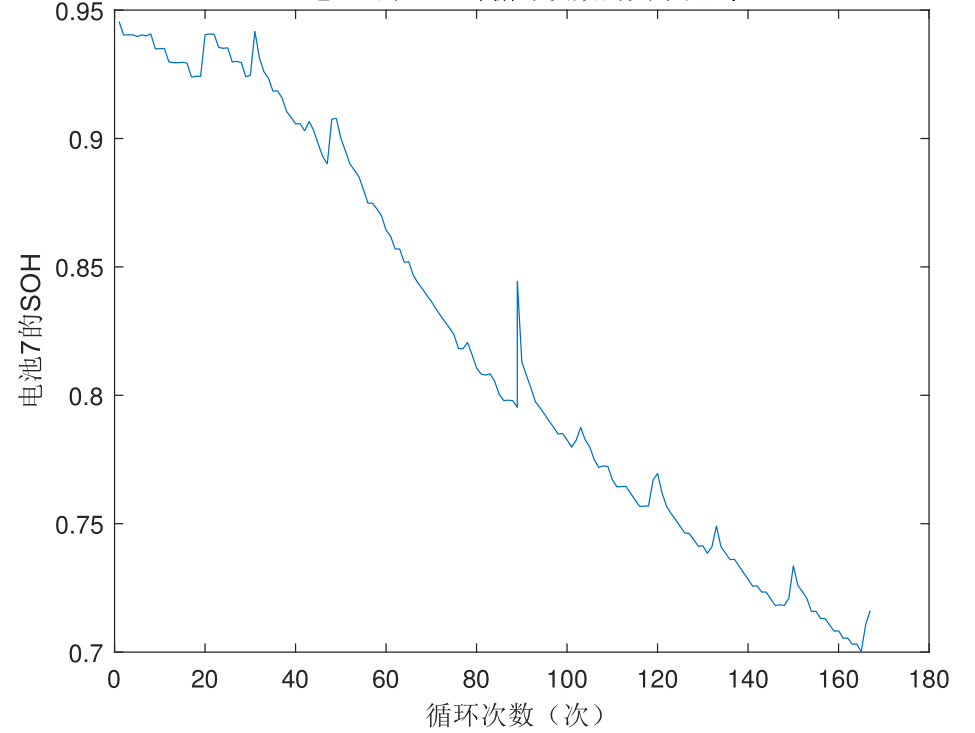
\includegraphics[width=0.8\textwidth]{img/7-SOH-cycle.png}
\caption{电池B0007的SOH与循环次数关系曲线}\label{figure-a}
\end{figure}

\newpage
在循环次数内,SOH值基本呈线性下降,属正常老化。同时,电池内阻随着循环次数增加而逐步增加,可得到如图所示结果:
\begin{figure}[H]
\centering
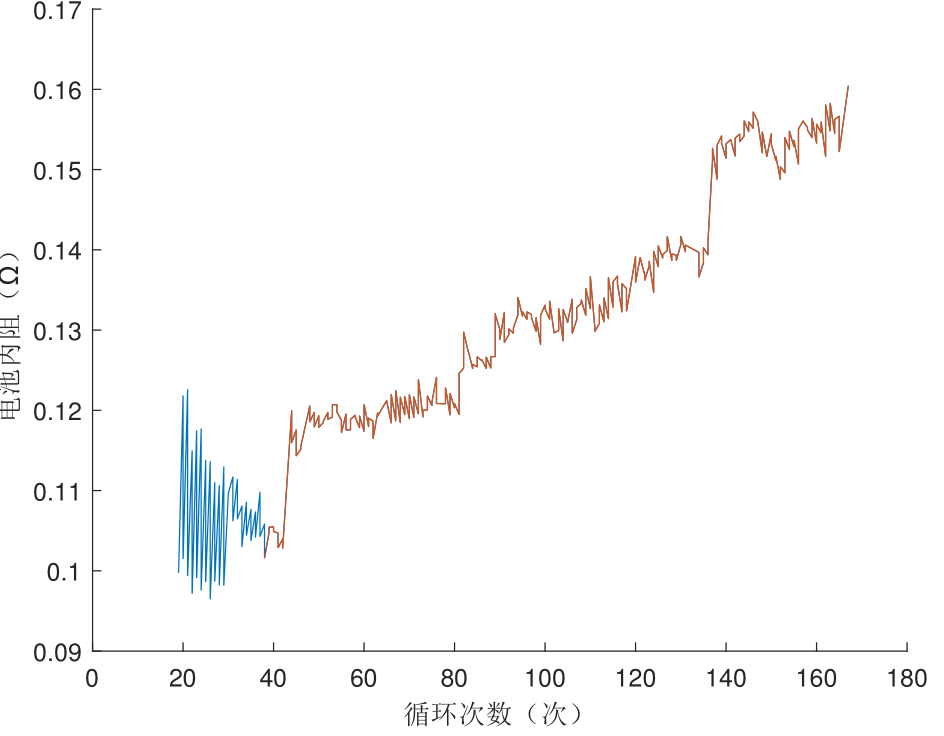
\includegraphics[width=0.8\textwidth]{img/R-cycle.png}
\caption{电池B0007的内阻与循环次数关系曲线}\label{figure-b}
\end{figure}

我们发现在电池循环前期,随着循环次数的增加,电池电阻缓慢下降,当循环试验进行到后期。随着循环次数的增加,电池内阻会有很大程度的下降。其中,前面波动较大是由于新电池刚开始充电时性能不稳定造成的,所以可把这一部分不考虑在内,只考虑循环后期电池状况稳定的情况。对余下曲线进行拟合,如图所示:\par
\begin{figure}[H]
\centering
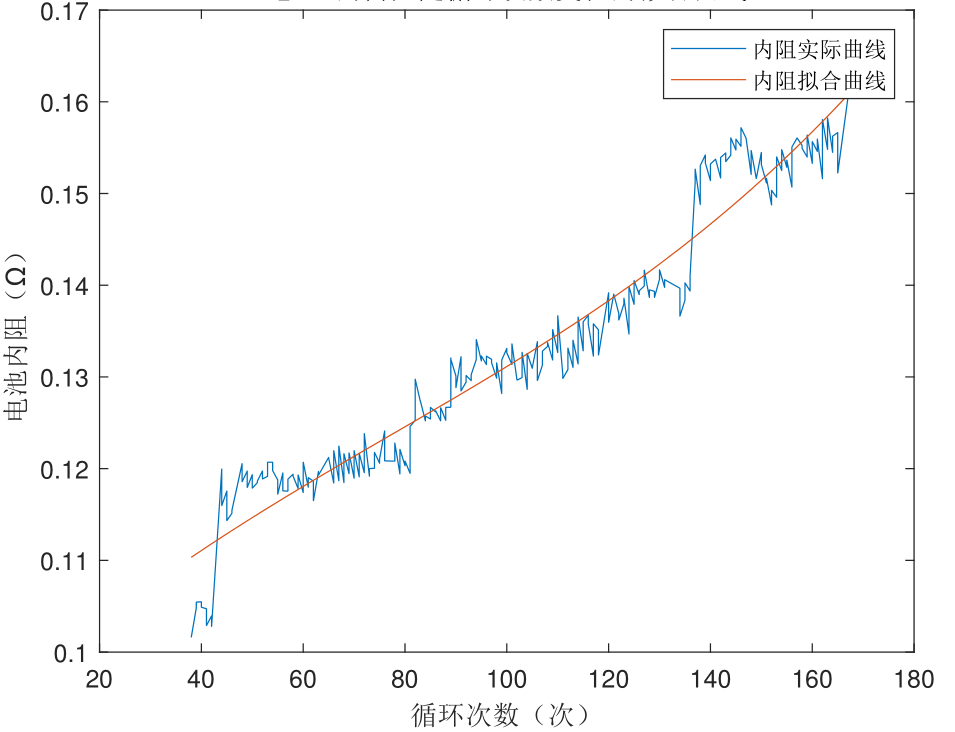
\includegraphics[width=0.8\textwidth]{img/R-cycle-fit.png}
\caption{电池B0007的内阻与循环次数的拟合曲线}
\end{figure}
该曲线与交流阻抗变化规律吻合,随着电池老化阻值不断增加。所以我们可认为在数据所给的循环次数内,电池处于正常老化区域。
所以,所给数据符合电化学阻抗谱法适用条件。


\subsection{问题二分析}



\section{问题的解答}
\subsection{问题1的解答}

我们用电阻测试结果表示SOH,可获得如图的SOH和电池电阻关系图,分析数据可知,电池SOH随着电阻老化呈单调下降,采用四次拟合的方法,我们可近似计算电池SOH老化规律曲线
\begin{figure}[H]
\centering
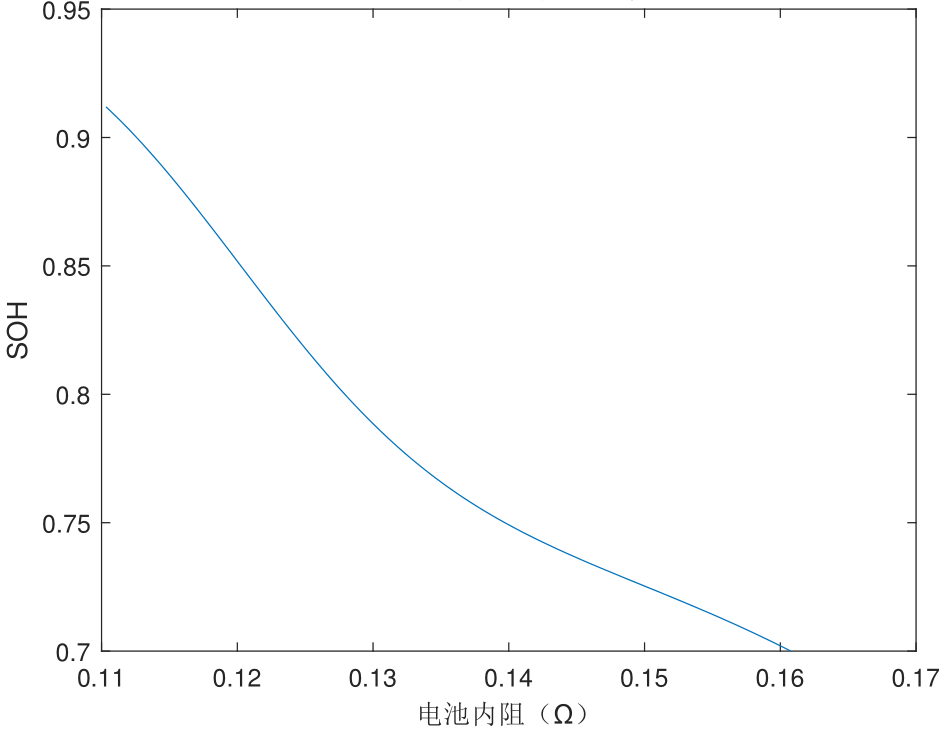
\includegraphics[width=0.8\textwidth]{img/SOH-R-fit.png}
\caption{电池B0007的SOH与其内阻变化曲线}
\end{figure}
通过MATLAB拟合求解,可得到相关系数为$0.9483$,表明电池内阻与电池SOH相关性较强,建立的模型具有一定的可靠性,可用该模型来预测B0005电池SOH。代入目标数据求得B0005预测SOH与真实值之间的均方根误差为$0.0296$


\subsection{问题2的解答}


\section{模型总结}

\subsection{模型优点}

\subsection{模型缺点}

\bibliographystyle{plain}
\bibliography{ref}
\begin{thebibliography}{99}
\bibitem{1}徐鑫珉、王练、史慧玲.基于电化学阻抗谱的电池老化寿命研究.电源技术.2018
\bibitem{2}丛巍.基于电化学阻抗模型的锂离子电池寿命预测研究.哈尔滨工业大学.2017
\bibitem{3} 
\end{thebibliography}

\newpage
\appendix
\textbf{附录}
\section{模型求解代码}

\end{document}
